%=========================================================================
% sec-opts-prof
%=========================================================================

\section{Utilizing Profile-Guided Optimization}
\label{sec-opts-prof}

% Reason for optimization
\subsection{Reason for Optimization}

Modern compilers are quite sophisticated and provide many features that
can improve the quality of the generated code. However, a general
challenge with compilers is that they can only act on static
analysis. This means that it cannot make any assumptions about
data-dependent control flow. If the compiler could have access to dynamic
information about an application, though, it could predicate branches
more aggressively based on the general patterns it detects during
runtime.
\smallskip

% Details of optimization
\subsection{Details of Optimization}

Fortunately, we can actually provide such dynamic information to the
compiler by using profile-guided optimizations (PGO). By enabling PGO in
the compiler, every run of an application dumps a .dyn file that
summarizes the trends of the application during runtime. This information
in turn can be used in a subsequent compilation to aggressively optimize
the code.
\smallskip

From our experiments, it seems that the more dynamic information is
collected in the form of multiple .dyn files, the more the performance
improves. This makes sense since with more samples, the compiler is
getting a more accurate portrayal of the average execution of the
application.
\smallskip

% Results and analysis
\subsection{Results}

%=========================================================================
% fig-opts-prof-results.tex
%=========================================================================

\begin{figure}[h]

  \centering
  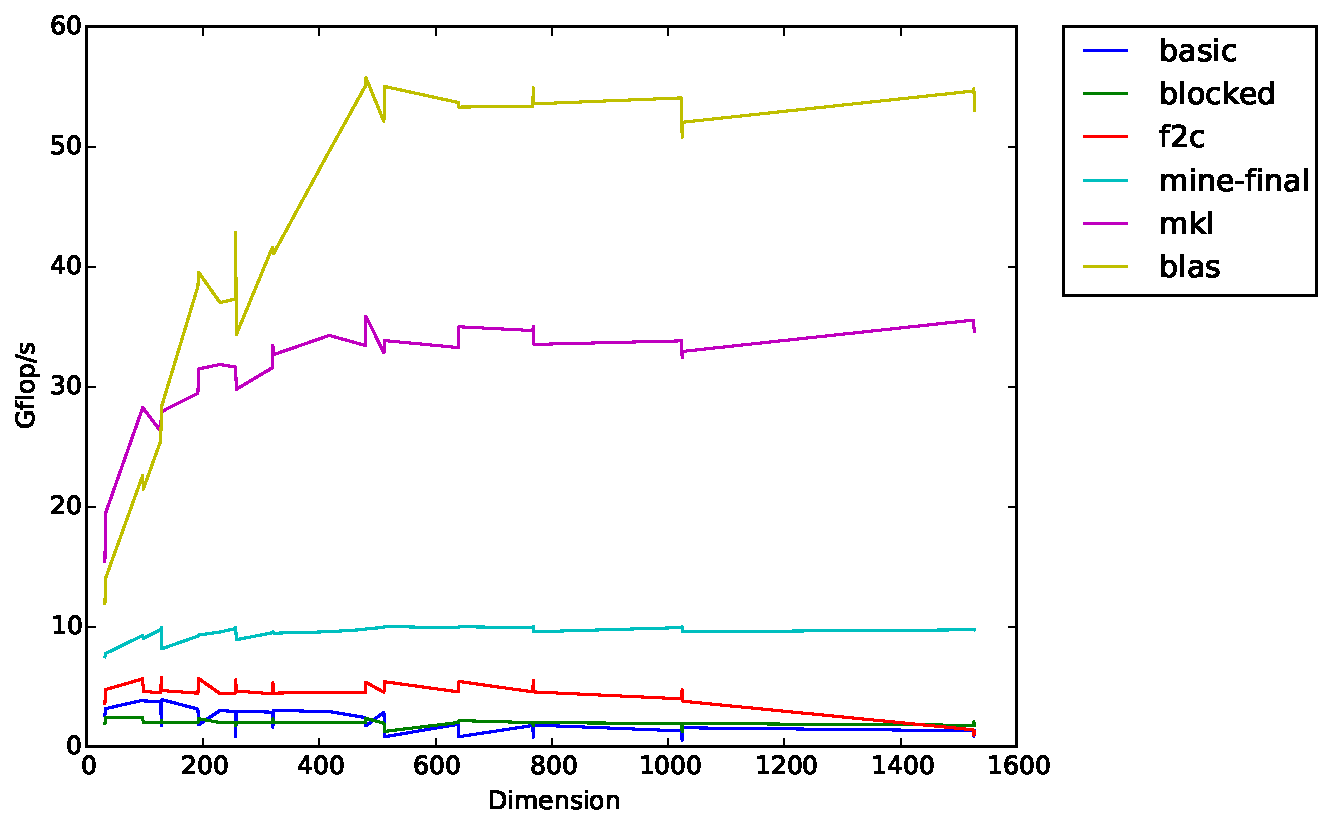
\includegraphics[width=0.7\tw]{fig-opts-prof-results.pdf}

  \caption{\textbf{Performance Comparison of PGO Optimizations --}
    Results for the final DGEMM implementation with all optimizations in
    this assignment, including the profile-guided optimization using data
    from ten unique .dyn files are shown compared against all provided
    implementations.}

  \label{fig-opts-prof-results}

\end{figure}


Figure~\ref{fig-opts-prof-results} shows the results with PGO enabled
using dynamic information collected from ten unique runs. Please see the
prof/ subdirectory for all .dyn files. The culmination
of all the optimizations explored in this assignment shows that we can
reach over 10GFLOPS/s of performance, which is roughly a 5x speedup over
the naive blocked baseline implementation.
